\section{Fourier: From Bad to Worse—The Existential Crisis of Mathematical Analysis (1822)}

\subsection{The Equation That Shook Mathematics: Fourier and the Waves Beneath Everything}

Just when mathematicians thought they had seen the worst of it, Jean-Baptiste Joseph Fourier came along and delivered another existential crisis.

In the early 19th century, Fourier was not trying to cause mathematical turmoil: he was simply trying to understand how heat flows (i.e. heat conduction). He was fascinated with how diffusion spreads an initial disturbance, and how that process can be described as the evolution of wave components with time-varying amplitudes.

At the heart of his method was what is now called a \textbf{Fourier series}. It was a way to express a function as an infinite sum of trigonometric functions:

\[
f(x) = a_0 + \sum_{n=1}^{\infty} \left( a_n \cos(n x) + b_n \sin(n x) \right).
\]

\begin{figure}[H]

\begin{center}
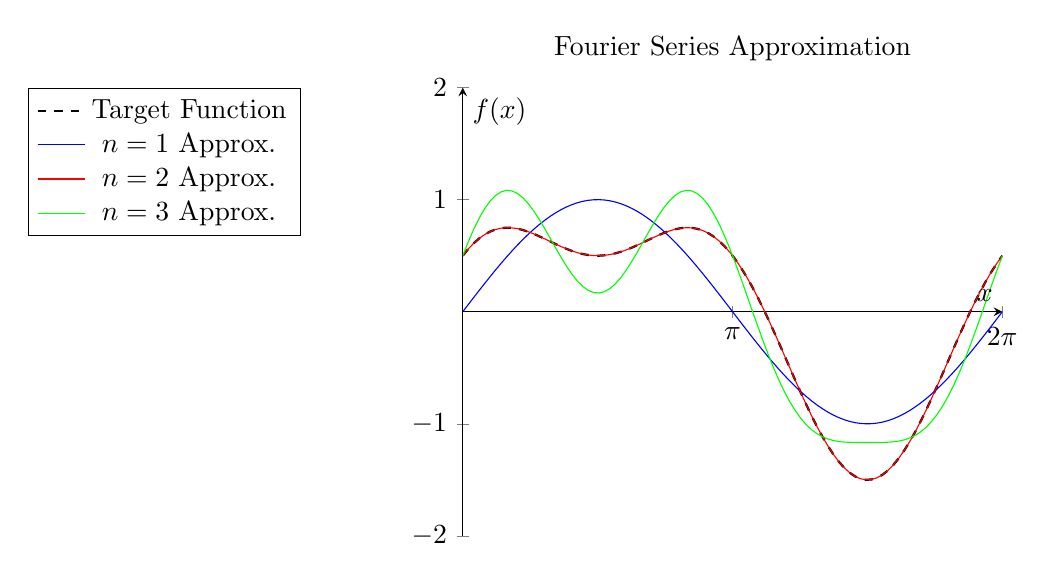
\begin{tikzpicture}
    \begin{axis}[
        domain=0:2*pi,
        samples=100,
        axis x line=middle,
        axis y line=middle,
        ymin=-2, ymax=2,
        xlabel={$x$}, ylabel={$f(x)$},
        xtick={0, 3.14, 6.28},
        xticklabels={$0$, $\pi$, $2\pi$},
        title={Fourier Series Approximation},
        legend style={at={(-0.3,1)}, anchor=north east} % Moves legend to the far left
    ]

        % Base function (target function)
        \addplot[thick, black, dashed, domain=0:2*pi] {sin(deg(x)) + cos(deg(2*x))/2};
        
        % First approximation (n=1)
        \addplot[blue, domain=0:2*pi] {sin(deg(x))};
        
        % Second approximation (n=2)
        \addplot[red, domain=0:2*pi] {sin(deg(x)) + cos(deg(2*x))/2};
        
        % Third approximation (n=3)
        \addplot[green, domain=0:2*pi] {sin(deg(x)) + cos(deg(2*x))/2 + sin(deg(3*x))/3};

        \legend{Target Function, $n=1$ Approx., $n=2$ Approx., $n=3$ Approx.}

    \end{axis}
\end{tikzpicture}
\end{center}
  \caption{PUT SOMETHING HERE}
\end{figure}


This equation says something remarkable: no matter how messy or irregular a function might seem, it could be reconstructed entirely from smooth waves. Fourier discovered that even functions describing complex heat distributions could be rewritten in this way, making it much easier to analyze how temperature evolved over time.


\subsection*{A Language for Change: What Differential Equations Tell Us}

Before we dive into the specific equations used by Fourier, we need to introduce one of the central tools of his work: the differential equation. 


Specifically, Fourier studied the \textit{heat equation}: a partial differential equation (PDE) describing how heat diffuses through a medium over time.

\[
\frac{\partial u}{\partial t} = \alpha \frac{\partial^2 u}{\partial x^2}
\]


Where:
\begin{itemize}
  \item \( u(x, t) \) is the temperature at position \( x \) and time \( t \),
  \item \( \alpha \) is the thermal diffusivity constant.
\end{itemize}

In the case of the heat equation, it tells us how the temperature \( u(x, t) \) changes over time (\( \frac{\partial u}{\partial t} \)) based on how curved or uneven the temperature is across space (\( \frac{\partial^2 u}{\partial x^2} \)). 

Solving this differential equation means figuring out what the temperature is at every point and time, given how it spreads and smooths out.

This isn’t just mathematical machinery: it’s a language for describing how physical systems change, either across space, over time, or both. Understanding this language, even at a basic level, will help us make sense of the ideas that follow.

A \textbf{differential equation} is an equation that relates a function to its derivatives; in other words, it describes how something is changing.

A \textbf{derivative} tells you how a quantity changes at each point. If you have a function for position, its derivative is velocity—how fast and in what direction the position is changing. A second derivative gives acceleration—how fast the velocity is changing.

An \textbf{integral}, by contrast, adds up small changes to find a total. If velocity is the derivative of position, then integrating velocity over time gives you the distance traveled.

A \textbf{differential equation} combines these ideas. It gives a rule that a function must follow—not just what a quantity is, but how it \textit{behaves} and \textit{evolves}. Solving a differential equation means finding a function whose derivatives fit that rule.

\begin{quote}
Think of a differential equation as a recipe for change. It doesn’t tell you what the answer is; it tells you how the answer must behave.
\end{quote}

When a differential equation involves more than one independent variable—such as time and space—it becomes a \textbf{partial differential equation}, or PDE. These equations describe how things evolve over both space \textit{and} time. They are the mathematical heart of waves, heat, gravity, fluids, and much more.

In the sections that follow, we’ll see how different PDEs capture two fundamental kinds of behavior: how systems evolve \textit{in time}, and how they are structured \textit{across space}.



\subsection{d’Alembert and the Wave Equation: Time in Motion}

In the mid-1700s, Jean le Rond d’Alembert studied the motion of vibrating strings and derived one of the earliest examples of what we now call a \textit{partial differential equation}: the wave equation.

In physical terms, a wave is any quantity that oscillates (i.e. it goes up and down over space or time), and they wave have these key features:

\begin{itemize}
  \item \textbf{Amplitude}: how tall the wave is — its maximum height from the center line.
  \item \textbf{Wavelength}: the horizontal distance over which the wave pattern repeats.
  \item \textbf{Frequency}: how many complete waves fit within a certain interval.
  \item \textbf{Phase}: the relative horizontal shift of a wave — it tells you where the wave starts in its cycle.
\end{itemize}

Sine waves are one of the simplest types, and they form the basic ingredients of more complex signals. It is an example of \textbf{trigonometric functions}, and they describe smooth, repeating wave patterns.

\begin{figure}[H]
  \centering

  % First row: Amplitude (left) and Wavelength (right)
  \begin{subfigure}[t]{0.45\textwidth}
    \centering
    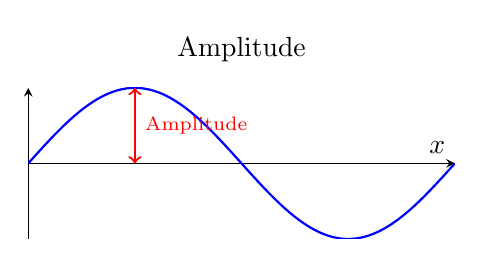
\begin{tikzpicture}
      \begin{axis}[
        axis lines = middle,
        xlabel = $x$,
        xtick=\empty,
        ytick=\empty,
        width=7cm,
        height=3.5cm,
        domain=0:2*pi,
        samples=200,
        title={Amplitude}
      ]
        \addplot[thick, blue] {sin(deg(x))};
        \draw[<->, red, thick] (axis cs:pi/2,0) -- (axis cs:pi/2,1) node[midway, right] {\scriptsize Amplitude};
      \end{axis}
    \end{tikzpicture}
    \caption{The vertical height from center to peak.}
  \end{subfigure}
  \hfill
  \begin{subfigure}[t]{0.45\textwidth}
    \centering
    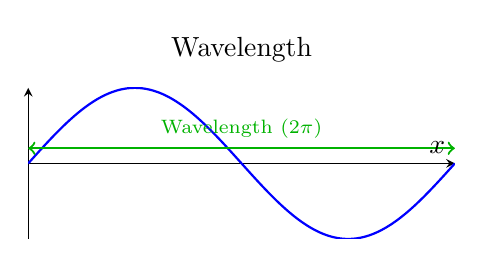
\begin{tikzpicture}
      \begin{axis}[
        axis lines = middle,
        xlabel = $x$,
        xtick=\empty,
        ytick=\empty,
        width=7cm,
        height=3.5cm,
        domain=0:2*pi,
        samples=200,
        title={Wavelength}
      ]
        \addplot[thick, blue] {sin(deg(x))};
        \draw[<->, green!70!black, thick] (axis cs:0,0.2) -- (axis cs:2*pi,0.2) node[midway, above] {\scriptsize Wavelength ($2\pi$)};
      \end{axis}
    \end{tikzpicture}
    \caption{The horizontal distance for one full cycle.}
  \end{subfigure}

  \vspace{0.8cm}

  % Second row: Frequency (left) and Phase (right)
  \begin{subfigure}[t]{0.45\textwidth}
    \centering
    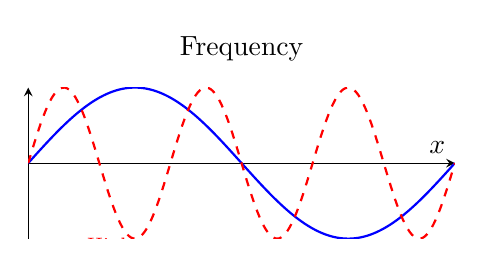
\begin{tikzpicture}
      \begin{axis}[
        axis lines = middle,
        xlabel = $x$,
        xtick=\empty,
        ytick=\empty,
        width=7cm,
        height=3.5cm,
        domain=0:2*pi,
        samples=200,
        title={Frequency}
      ]
        \addplot[thick, blue] {sin(deg(x))};
        \addplot[thick, red, dashed] {sin(deg(3*x))};
        \node[blue] at (axis cs:1.2,1.1) {\scriptsize Low};
        \node[red] at (axis cs:1.2,-1.1) {\scriptsize High};
      \end{axis}
    \end{tikzpicture}
    \caption{More cycles = higher frequency.}
  \end{subfigure}
  \hfill
  \begin{subfigure}[t]{0.45\textwidth}
    \centering
    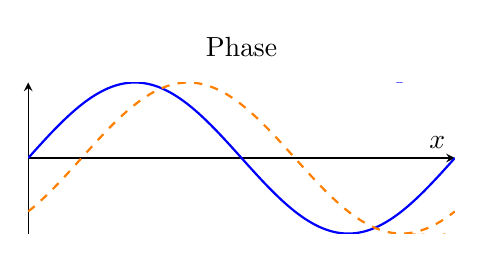
\begin{tikzpicture}
      \begin{axis}[
        axis lines = middle,
        xlabel = $x$,
        xtick=\empty,
        ytick=\empty,
        width=7cm,
        height=3.5cm,
        domain=0:2*pi,
        samples=200,
        title={Phase}
      ]
        \addplot[thick, blue] {sin(deg(x))};
        \addplot[thick, orange, dashed] {sin(deg(x - pi/4))};
        \node[blue] at (axis cs:5.5,1.1) {\scriptsize Original};
        \node[orange] at (axis cs:6.1,-1.1) {\scriptsize Shifted};
      \end{axis}
    \end{tikzpicture}
    \caption{Phase shift moves the wave left or right.}
  \end{subfigure}

  \caption{The four basic properties of waves: amplitude, wavelength, frequency, and phase.}
\end{figure}




To begin, we define the function \textbf{\( u(x, t) \) as \textit{vertical displacement} of a point on the string at position \( x \) and time \( t \)}. In other words, \( u(x, t) \) tells us how much the string is displaced from its equilibrium position at a given location \( x \) and time \( t \). 


\begin{figure}[H]
  \centering
  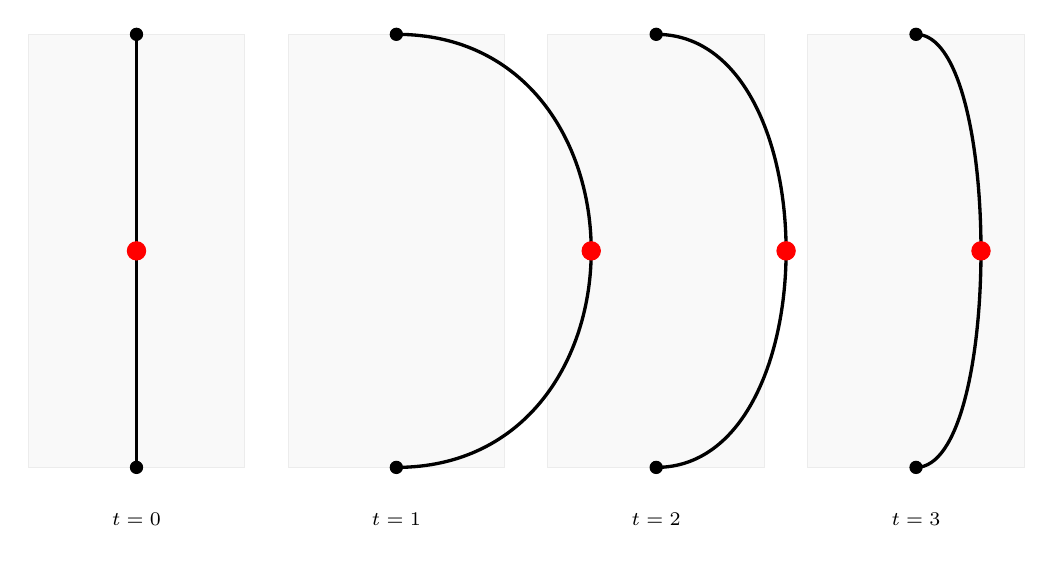
\begin{tikzpicture}[scale=1.1]

    % Constants
    \def\topY{2.5}
    \def\midY{0}
    \def\botY{-2.5}
    \def\panelWidth{2.5}

    % === First Pass: Draw all panel backgrounds and fixed points ===
    \foreach \xshift/\timeLabel in {
      0/0,
      3/1,
      6/2,
      9/3
    } {
      \begin{scope}[xshift=\xshift cm]
        % Background rectangle
        \draw[gray!15, fill=gray!05] (-\panelWidth/2,\botY) rectangle (\panelWidth/2,\topY);

        % Fixed endpoints
        \filldraw[black] (0,\topY) circle (2pt);
        \filldraw[black] (0,\botY) circle (2pt);

        % Time label
        \node at (0,\botY - 0.6) {\scriptsize $t = \timeLabel$};
      \end{scope}
    }

    % === Second Pass: Draw Bézier curves and manually placed red dots ===
    % Format: xshift / control point x / red dot x
    \foreach \xshift/\ctrlX/\redX in {
      0/0/0,
      3/3/2.25,
      6/2/1.5,
      9/1/0.75
    } {
      \begin{scope}[xshift=\xshift cm]
        % Bézier curve
        \draw[very thick] (0,\topY)
          .. controls (\ctrlX,\topY) and (\ctrlX,\botY) ..
          (0,\botY);

        % Manually placed red dot at height = 0
        \filldraw[red] (\redX,\midY) circle (3pt);
      \end{scope}
    }

  \end{tikzpicture}
  \caption{Manual version: each panel shows a vertical string with fixed endpoints (black dots). The Bézier curve shape is controlled via control points, and the red dot is placed manually to show the displacement \( u(x, t) \).}
\end{figure}

\vspace{1.5em}


The displacement changes over time in an oscillating fashion. The motion this vibrating string describes the displacement that varies over both space and time, and the wave equation models how this displacement evolves.

\begin{figure}[H]
\centering
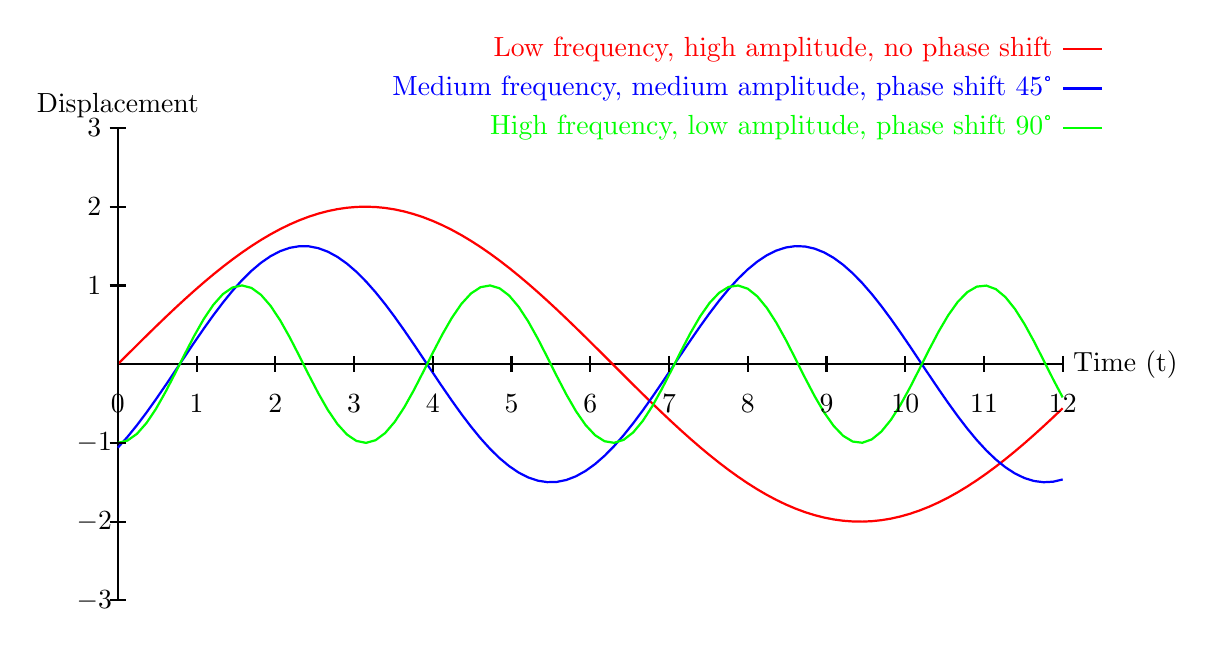
\begin{tikzpicture}

% Draw the x-axis (time axis)
\draw[thick] (0,0) -- (12,0) node[right] {Time (t)};

% Draw the y-axis (displacement axis)
\draw[thick] (0,-3) -- (0,3) node[above] {Displacement};

% Draw waveforms with different frequencies, amplitudes, and wavelengths, with phase shifts

% Wave with low frequency (longer wavelength), no phase shift
\draw[thick, red] plot[domain=0:12,samples=100] (\x,{2*sin(0.5*\x r)}) node[pos=1, above right] {};

% Wave with medium frequency and medium amplitude, with phase shift of 45 degrees
\draw[thick, blue] plot[domain=0:12,samples=100] (\x,{1.5*sin(1*\x r - 45)}) node[pos=1, above right] {};

% Wave with high frequency (shorter wavelength), with phase shift of 90 degrees
\draw[thick, green] plot[domain=0:12,samples=100] (\x,{1*sin(2*\x r - 90)}) node[pos=1, above right] {};

% Adding tick marks for position x on the x-axis (time intervals)
\foreach \x in {0, 1, 2, 3, 4, 5, 6, 7, 8, 9, 10, 11, 12} {
    \draw[shift={(\x,0)}, thick] (0,3pt) -- (0,-3pt);
    \node at (\x,-0.5) {$\x$};
}

% Adding tick marks for position y on the y-axis (displacement)
\foreach \y in {-3,-2,-1,1,2,3} {
    \draw[shift={(0,\y)}, thick] (-3pt,0) -- (3pt,0);
    \node at (-0.3,\y) {$\y$};
}

% Legend for frequency, amplitude, wavelength, and phase shift
\draw[thick, red] (12.5,4) -- (12,4)  node[left] {Low frequency, high amplitude, no phase shift};
\draw[thick, blue]  (12.5,3.5) -- (12,3.5) node[left] {Medium frequency, medium amplitude, phase shift 45°};
\draw[thick, green]  (12.5,3) -- (12,3) node[left] {High frequency, low amplitude, phase shift 90°};

\end{tikzpicture}
\caption{Illustration of different waveforms with varying frequencies, amplitudes, wavelengths, and phase shifts. The red curve represents a wave with low frequency and high amplitude, with no phase shift. The blue curve represents a wave with medium frequency and amplitude, with a phase shift of 45°. The green curve represents a wave with high frequency and low amplitude, with a phase shift of 90°. The legend explains the characteristics of each wave.}
\end{figure}

\vspace{1.5em}


In the context of a vibrating string, these wave properties are not just abstract concepts — they’re fundamental to how the wave behaves and how the PDE is solved.

To get an intuitive feel for this, imagine plucking a taut string like on a guitar. The shape of the wave that travels down the string depends on 

\begin{enumerate}
	\item how hard you pull it \textbf{(amplitude)}, 
	\item how tightly the string is held (which affects \textbf{frequency and wavelength}), 
	\item and exactly where and when you let go (which influences the \textbf{phase}). 
\end{enumerate}
	
The motion that follows can be predicted and described using the wave equation — a mathematical way of capturing that energy rippling back and forth through the string.


\subsection{Explanation of Frequency, Amplitude, Wavelength, Phase Shift, and Partial Differential Equations}


\subsubsection{Frequency}

Frequency refers to how many complete oscillations a wave undergoes per unit time. For a vibrating string—like one on a guitar—frequency determines the pitch you hear. Pluck the string gently or press it down at a different fret, and the number of vibrations per second changes. That change in vibration rate is a change in frequency.

Mathematically, frequency appears in the \textit{temporal part} of the wave solution, \( T_n(t) \), and governs how fast the wave oscillates in time at a fixed location. But how do we represent these oscillations?

This is where trigonometry begins to enter the picture in earnest. Sine and cosine functions are the mathematical language of oscillations. Their smooth, repeating behavior makes them perfect tools for modeling how the string moves up and down over time.

A basic wave at a point can be described using a function like:
\[
T_n(t) = \cos(\omega_n t)
\]
Here, \( \omega_n \) is the \textit{angular frequency}, which is directly related to how rapidly the wave cycles. This function tells us how the vertical position of a single point on the string changes as time goes on—exactly the kind of information we care about when thinking of sound waves, music, and vibration.

When you press a fret on a guitar, you shorten the effective length of the string, which changes the boundary conditions and leads to a higher natural frequency. Trigonometric functions help us describe this change quantitatively. The faster the wave cycles (i.e., the higher the frequency), the more tightly packed the sine or cosine wave becomes on a graph

    
\subsubsection{Amplitude}

The amplitude refers to the maximum displacement of the string from its equilibrium position. In physical terms, it represents how far the string moves from rest at its most extreme point. On a guitar, this corresponds to how hard you pluck the string — a gentle pluck produces a small amplitude (a soft sound), while a hard pluck creates a larger amplitude (a louder sound).

In the mathematical solution to the wave equation, amplitude is determined by the constants \( A_n \) and \( B_n \), which scale the temporal solution. These constants determine the height of the wave and stay fixed as the wave propagates, assuming no energy loss (i.e., no damping).

To describe these oscillations precisely, we again turn to trigonometric functions like sine and cosine. For instance, a point on the string moving in time might be described by:
\[
T_n(t) = A_n \cos(\omega_n t) + B_n \sin(\omega_n t)
\]
Here, \( A_n \) and \( B_n \) control the amplitude — how high or low the wave goes — while \( \omega_n \) (the angular frequency) controls how fast it oscillates. The sum of sine and cosine terms reflects the wave's shape and initial conditions, and it allows us to capture both the height and timing of the vibration.

Visually, the amplitude is the vertical "reach" of the wave from the centerline. On the guitar, the amplitude of the vibrating string maps directly to the volume of the sound produced — a visible motion with audible consequences.

In the next section, we’ll look more closely at how these sine and cosine functions work, and how they form the building blocks of wave solutions.
    
\subsubsection{Wavelength}

Wavelength is the spatial length over which the wave pattern repeats. On a guitar string, it corresponds to the distance between repeating peaks or troughs along the string’s length — the physical size of one complete "wave" on the string at a frozen moment in time.

The spatial variation of the wave is captured by the spatial part of the solution:
\[
X_n(x) = \sin\left(\frac{n\pi x}{L}\right)
\]
This is a sine function — one of the foundational objects in trigonometry — and it models the shape of the string in space. The variable \( x \) represents the position along the string, \( L \) is the total string length, and the integer \( n \) counts the harmonic mode (i.e., how many half-wavelengths fit along the string).

Each value of \( n \) gives a different standing wave pattern — these are the distinct musical notes you hear when pressing different frets. As \( n \) increases, the wavelength gets shorter, and the wave fits more "bumps" along the string. This reflects a crucial relationship in wave physics: wavelength is inversely related to frequency. Shorter wavelengths correspond to higher-frequency vibrations, which produce higher-pitched sounds.

In terms of trigonometry, the sine function \( \sin\left(\frac{n\pi x}{L} \right) \) repeats every \( \frac{2L}{n} \), so the wavelength for the \( n \)-th harmonic is:
\[
\lambda_n = \frac{2L}{n}
\]
As we go to higher harmonics, more oscillations fit into the same length of string — just like how playing a higher fret shortens the vibrating length and raises the pitch.

Wavelength, frequency, and amplitude are all woven together in the language of trigonometry, and together they shape the sound and motion of a vibrating string.

\subsubsection{Phase Shift}

Phase shift refers to how much a wave is shifted along the horizontal axis — that is, how "out of sync" it is compared to another wave. On a vibrating string, this can be thought of as a timing offset: when exactly does the motion at a particular point begin its oscillation?

Mathematically, the phase shift appears inside the argument of the temporal solution:
\[
T_n(t) = \cos(\omega_n t + \phi_n)
\]
Here, \( \phi_n \) is the \textit{phase shift}, and it determines the starting position of the oscillation in time. If two waves have the same frequency and amplitude but different phase shifts, they follow the same path — just offset in time. 

Returning to the guitar analogy, imagine plucking two identical strings at different moments. The waves they generate have the same shape and speed, but one starts just a little later than the other. That delay is a phase shift. Even if the strings vibrate with the same frequency and amplitude, the sound wave might be slightly out of alignment — which, in the case of multiple strings playing together, can create interesting interference patterns (or sometimes, dissonance!).

Trigonometry captures this effect naturally. Both sine and cosine functions allow for horizontal shifts built directly into their arguments:
\[
\sin(\omega t + \phi) \quad \text{or} \quad \cos(\omega t + \phi)
\]
Changing \( \phi \) slides the graph left or right without altering its shape — the frequency, amplitude, and wavelength all stay the same. This flexibility makes trigonometric functions ideal for modeling time-dependent behaviors like wave motion.

In musical terms, the phase shift doesn’t change the pitch or volume — just when the note begins to sound. And in mathematical terms, it gives us precise control over wave timing, which becomes especially powerful when we start combining waves to form complex signals.

\subsubsection{Partial Differential Equations}

Together, amplitude, frequency, wavelength, and phase describe the fundamental behavior of waves on a vibrating string. These properties are not just abstract descriptors — they’re built directly into the mathematical structure of the wave.

The full wave function \( u(x, t) \), which represents the displacement of the string at a position \( x \) and time \( t \), is typically written as a product of two components:
\[
u(x, t) = X_n(x) \cdot T_n(t)
\]
The spatial part \( X_n(x) \) captures the standing wave pattern along the length of the string, while the temporal part \( T_n(t) \) tracks how that pattern evolves over time.

Each of these components is shaped by trigonometric functions — sine and cosine — which naturally model periodic, oscillatory motion. Amplitude appears as a scaling factor, frequency is encoded in the wave’s angular velocity \( \omega_n \), wavelength determines the spacing of the wave in space, and phase shift adjusts its timing. These ingredients define how the wave looks and sounds — much like how a guitar string’s pitch and tone depend on how and where it’s plucked.

All of this behavior is governed by a \textbf{partial differential equation (PDE)} — specifically, the wave equation:
\[
\frac{\partial^2 u}{\partial t^2} = c^2 \frac{\partial^2 u}{\partial x^2}
\]
This equation links the second derivative of \( u(x, t) \) with respect to time (how fast the acceleration of the wave changes) to its second derivative with respect to space (how curved the string is at each point). The constant \( c \) represents the wave speed along the string.

In essence, the wave equation encodes how the string’s shape and motion evolve in tandem — how energy moves, bounces, and ripples. It’s the mathematical heart of vibration and sound. Through this equation, and with the help of trigonometry, we begin to see how the language of waves is not just visual or physical — it is deeply mathematical.

In the next section, we’ll see how solving this PDE leads us into deeper territory: eigenfunctions, boundary conditions, and the emergence of harmonics.
















\subsection{Solving the Wave Equation}

\subsubsection{Initial and Boundary Conditions: Setting the Stage for Vibration}

To explore these concepts in action, we now turn to solving the wave equation for a specific physical system: a stretched string of fixed length \( L \), held tightly at both ends. Mathematically, this means we enforce boundary conditions \( u(0,t) = u(L,t) = 0 \) for all times \( t \). These conditions represent the fact that the ends of the string are pinned down and cannot move — like a guitar string fastened at both ends.

But to fully describe how the string will move, we also need to know how it started. The wave equation doesn’t act in isolation — it evolves whatever situation it begins with. That’s where the initial conditions come in:
\[
u(x,0) = f(x), \quad \left.\frac{\partial u}{\partial t}\right|_{t=0} = g(x)
\]

The function \( f(x) \) tells us the shape of the string at the starting moment — perhaps it was pulled into a triangle, bowed into a curve, or left flat. The function \( g(x) \) tells us how each point on the string was moving at that initial moment — whether it was released from rest, struck with a pulse, or already oscillating.

Together, these initial and boundary conditions define the entire story. The wave equation then becomes a kind of “motion engine,” calculating how the shape evolves from this starting point, honoring both the physical constraints (fixed endpoints) and the initial motion.

Solving this problem means uncovering how a specific, physical setup gives rise to complex but predictable waves — the kind of patterns we see every time we strum a stringed instrument or observe ripples in a stretched surface.


\subsubsection{The Wave Equation:}
\[
\frac{\partial^2 u}{\partial t^2} = c^2 \frac{\partial^2 u}{\partial x^2}
\]

The wave equation models how a string moves as it vibrates. Here, \( u(x, t) \) represents the vertical displacement of the string at position \( x \) and time \( t \). On the left-hand side, \( \frac{\partial^2 u}{\partial t^2} \) is the \textit{acceleration} — how quickly the position of the string is changing over time. On the right-hand side, \( \frac{\partial^2 u}{\partial x^2} \) is the \textit{curvature} — a measure of how sharply the string is bending at that point in space.

This equation tells us that the acceleration of a point on the string depends entirely on its curvature. That is: \textit{a point will only start to move (speed up or slow down) if it’s part of a bend}. If the string is flat at that point — no curvature — then there’s no reason for it to accelerate.

Think of the string like a flexible ruler. If it’s completely flat, and you let go, nothing happens. But if you bend it and then release, the curved part snaps back — the tighter the curve, the stronger the snap. The wave equation captures this exact idea: curves cause motion.

The constant \( c \) represents the wave speed — how fast the disturbance travels through the string. So this equation shows that any bump or bend in the string doesn’t just stay in place — it causes neighboring points to accelerate, spreading the motion outward as a wave.

In this way, the wave equation beautifully links geometry (how bent the string is) to dynamics (how fast each point moves), showing how ripples travel through space over time.


\subsubsection{Assume Form: }

\[
u(x,t) = X(x)T(t)
\]

When faced with a complex system like a vibrating string, the wave equation involves both space and time — meaning we’re trying to understand how the shape of the string changes at every point in space, at every moment in time. That’s a lot to handle at once.

To make the problem manageable, we assume something powerful: that the full motion can be broken into two simpler parts — one that only describes how the string bends in space (\( X(x) \)), and another that only describes how that shape pulses over time (\( T(t) \)).

This assumption may seem bold, but it’s not arbitrary. In physical systems with symmetry and regular boundary conditions (like fixed ends on a string), it turns out that these space-time patterns often *do* separate cleanly. It’s like analyzing a musical note — we can study the pitch (which depends on vibration frequency) separately from the waveform (the pattern of the vibration).

Writing the solution as a product \( u(x,t) = X(x)T(t) \) turns a two-variable problem into two one-variable problems. Instead of trying to analyze a swirling, dancing motion all at once, we split it into:  
- **Where** the string can move (its shape), and  
- **How** that motion changes over time.

This idea — to assume a separable form — is the first step that unlocks the rest of the solution method. Without it, we’d be left trying to untangle a knot of partial derivatives across both dimensions at once.

\subsubsection{Separate Variables:}
\[
\frac{T''(t)}{c^2 T(t)} = \frac{X''(x)}{X(x)} = -\lambda
\]

To understand the motion of a vibrating string, we’re trying to solve a wave equation that depends on both space (\(x\)) and time (\(t\)). But solving a function of two variables can be messy — unless we assume something helpful: what if the solution can be written as a product of two separate parts, one depending only on space and the other only on time?

This is the core idea behind \textit{separation of variables}. We assume:
\[
u(x, t) = X(x) T(t)
\]
This is like saying: "Let’s break down the complex motion of the string into simpler components — one part that tells us the shape of the string, and another that tells us how that shape evolves over time."

When we plug this product into the wave equation and divide both sides by \(X(x)T(t)\), something elegant happens: all the time-dependent stuff ends up on one side, and all the space-dependent stuff ends up on the other. Since these two sides depend on entirely different variables, the only way this equation can be true for *every* \(x\) and *every* \(t\) is if they both equal the same constant — which we call \( -\lambda \).

That split gives us two separate ODEs:
\[
X''(x) + \lambda X(x) = 0 \quad \text{(spatial behavior)}
\]
\[
T''(t) + \lambda c^2 T(t) = 0 \quad \text{(temporal behavior)}
\]

Now, instead of one hard problem in two variables, we have two simpler problems — each in just one variable. This is like trying to understand a dance performance by analyzing the choreography (the pattern in space) and the rhythm (how fast and when it repeats) separately. The beauty is that the full motion can be reconstructed by multiplying the two: shape \(\times\) motion = vibration.

\subsubsection{Two ODEs:}
\[
X'' + \lambda X = 0 \quad \text{and} \quad T'' + \lambda c^2 T = 0
\]

These two differential equations describe two sides of the same story: how a vibrating string moves in space and time. The first equation, \( X'' + \lambda X = 0 \), governs the shape the string can take at any moment — this is the \textit{spatial behavior}. It tells us how the string bends, where the peaks and troughs can form, and what “shapes” are possible under the constraint of fixed endpoints. These shapes aren’t arbitrary: they’re the result of balancing the internal forces in the string, and only specific wave patterns — called \textit{modes} — are allowed.

Think of \( X(x) \) as a snapshot of the string, frozen in time. This equation defines what those snapshots are allowed to look like: how many wiggles (or nodes) the string can have, and where they must occur.

The second equation, \( T'' + \lambda c^2 T = 0 \), controls the \textit{temporal behavior} — how the amplitude of each mode rises and falls as time passes. This is the rhythm of the vibration. Every mode has its own natural frequency, determined by the same parameter \( \lambda \), and they each oscillate like a simple harmonic oscillator. If the spatial solution tells you the “shape” of the dance, then the temporal solution tells you how that shape sways in time.

Together, these equations describe standing waves: patterns that stay in place but pulse with time, like a jump rope held at both ends and wiggled just right to create a smooth, repeating ripple.


\subsubsection{ODE Solutions:}

\[
X_n(x) = \sin\left(\frac{n\pi x}{L}\right)
\quad \text{and} \quad
T_n(t) = A_n \cos\left(\frac{n\pi c t}{L}\right) + B_n \sin\left(\frac{n\pi c t}{L}\right)
\]

The solutions to these equations represent \textit{standing waves} — patterns of vibration that appear to oscillate in place, rather than traveling through space. Imagine a guitar string fixed at both ends. When plucked, the string doesn't just move randomly; it vibrates in distinct patterns called \textit{modes}. These modes are not arbitrary — they are the only possible shapes the string can sustain while still satisfying the boundary conditions.

The function \( X_n(x) \) describes these allowable shapes in space. Each value of \( n \) corresponds to a different \textit{mode shape} — the first mode (\( n = 1 \)) is the fundamental: a simple arc with no internal nodes except the fixed ends. Higher modes (\( n = 2, 3, \ldots \)) introduce more nodes, where the string doesn’t move at all. You can think of these as the natural "dance steps" that the string is allowed to perform.

Meanwhile, \( T_n(t) \) captures the rhythm of the dance — how each mode pulses in and out over time. It’s a combination of sine and cosine functions, meaning that each mode oscillates smoothly back and forth with a frequency proportional to \( n \). This frequency increases with the mode number: higher modes vibrate faster, just like tighter or shorter strings on an instrument produce higher-pitched notes.

Together, the spatial and temporal solutions describe how the string vibrates over space and time — a standing wave that wiggles, but never travels.


\subsubsection{Full Solution:}
\[
u(x,t) = \sum_{n=1}^{\infty} \left[ A_n \cos\left(\frac{n\pi c t}{L}\right) + B_n \sin\left(\frac{n\pi c t}{L}\right) \right] \sin\left(\frac{n\pi x}{L}\right)
\]

This expression is the full solution to the vibrating string problem — and it tells a complete story.

Instead of trying to describe the string’s motion with a single shape or frequency, we build the solution as a \textit{sum} of all the possible ways the string can vibrate. Each term in the sum represents a specific \textit{mode} of vibration: a distinct standing wave pattern that fits perfectly between the two fixed ends of the string.

The sine function \( \sin\left(\frac{n\pi x}{L}\right) \) gives the shape of the \( n^\text{th} \) mode in space — how many “humps” or nodes appear along the string. The functions of time (the sine and cosine terms) describe how that mode vibrates over time, pulsing rhythmically at its own natural frequency.

The constants \( A_n \) and \( B_n \) determine how much of each mode is present at the start — how strongly each one is "excited" when the string is first plucked or struck. These coefficients are determined by the initial shape and motion of the string, and they’re calculated using a method called a \textit{Fourier series}, which allows us to decompose any starting condition into a weighted sum of sine waves.

So in total, this solution is like building a complex musical tone by combining pure notes (the modes), each with its own pitch and intensity. The result is a rich, dynamic wave that captures every nuance of the string’s vibration.






\subsection{Smoothing the World: Heat, Harmonics, and the Birth of Fourier Analysis}

Now, let's come back to Fourier's heat equation:

\[
\frac{\partial u}{\partial t} = \alpha \frac{\partial^2 u}{\partial x^2}
\]


This tells us how the temperature \( u(x, t) \) changes over time (\( \frac{\partial u}{\partial t} \)) based on how curved or uneven the temperature is across space (\( \frac{\partial^2 u}{\partial x^2} \)). 

Solving a differential equation means figuring out what the temperature is at every point and time, given how it spreads and smooths out.

\begin{figure}[H]
\centering
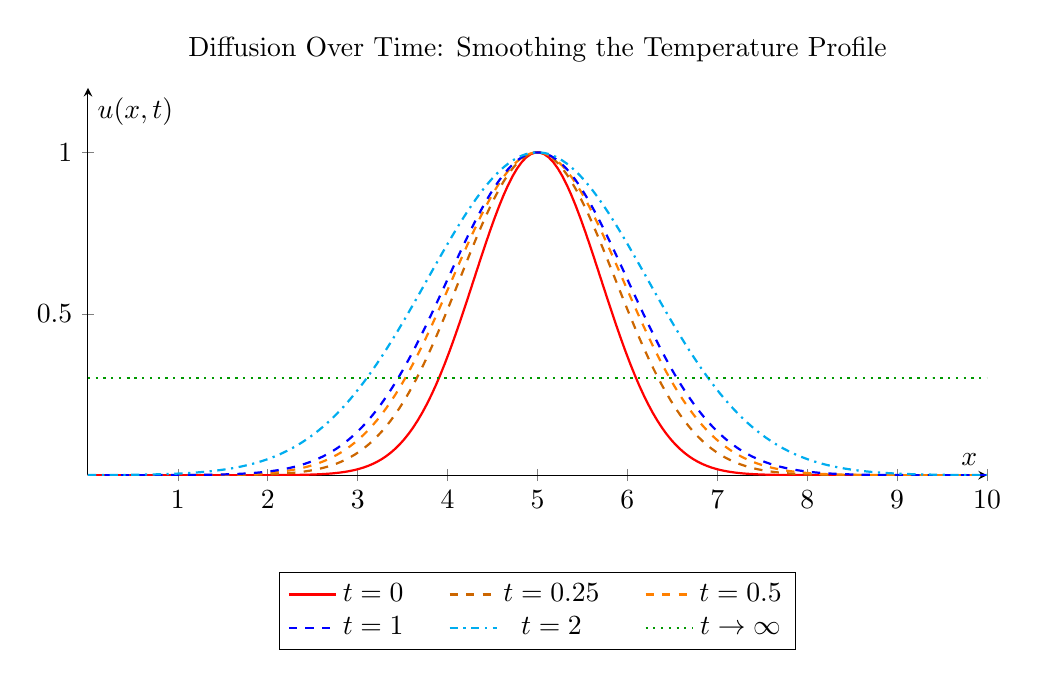
\begin{tikzpicture}
  \begin{axis}[
    domain=0:10,
    samples=200,
    axis lines = middle,
    xlabel = {$x$},
    ylabel = {$u(x, t)$},
    xmin=0, xmax=10,
    ymin=0, ymax=1.2,
    width=13cm,
    height=6.5cm,
    legend style={
      at={(0.5,-0.25)},
      anchor=north,
      legend columns=3,
      /tikz/every even column/.append style={column sep=0.5cm}
    },
    title={Diffusion Over Time: Smoothing the Temperature Profile}
  ]

    % t = 0
    \addplot[thick, red] {exp(-((x-5)^2))};
    \addlegendentry{$t = 0$}

    % t = 0.25
    \addplot[thick, orange!80!black, dashed] {exp(-((x-5)^2)/1.5)};
    \addlegendentry{$t = 0.25$}

    % t = 0.5
    \addplot[thick, orange, dashed] {exp(-((x-5)^2)/1.8)};
    \addlegendentry{$t = 0.5$}

    % t = 1
    \addplot[thick, blue, dashed] {exp(-((x-5)^2)/2)};
    \addlegendentry{$t = 1$}

    % t = 2
    \addplot[thick, cyan, dashdotted] {exp(-((x-5)^2)/3)};
    \addlegendentry{$t = 2$}

    % t → ∞
    \addplot[thick, green!60!black, dotted] {0.3};
    \addlegendentry{$t \rightarrow \infty$}

  \end{axis}
\end{tikzpicture}
\caption{The heat equation smooths out temperature differences over time. An initial sharp spike gradually diffuses and levels into a uniform profile.}
\end{figure}




To solve this kind of differential equation, Fourier looked for functions whose behavior under differentiation was easy to predict. He noticed that sine and cosine functions are especially convenient: when you take their second derivative, you simply get the same function back (up to a negative constant). For example:

\[
\frac{d^2}{dx^2} \sin(nx) = -n^2 \sin(nx)
\]

This property made sines and cosines ideal building blocks for constructing solutions to the heat equation.

\begin{figure}[H]
\centering
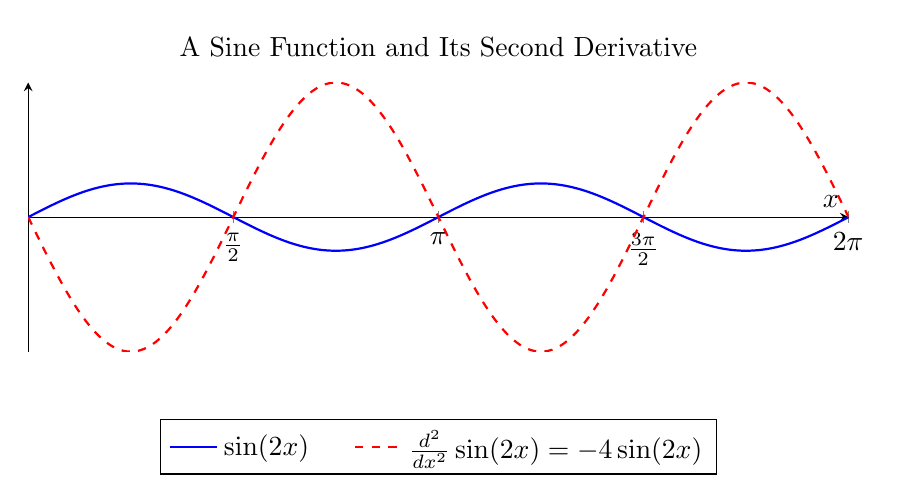
\begin{tikzpicture}
  \begin{axis}[
    domain=0:2*pi,
    samples=200,
    axis lines=middle,
    xlabel={$x$},
    ylabel={},
    xtick={0, 1.57, 3.14, 4.71, 6.28},
    xticklabels={$0$, $\frac{\pi}{2}$, $\pi$, $\frac{3\pi}{2}$, $2\pi$},
    ytick=\empty,
    width=12cm,
    height=5cm,
    legend style={
      at={(0.5,-0.25)},
      anchor=north,
      legend columns=2,
      /tikz/every even column/.append style={column sep=0.5cm}
    },
    title={A Sine Function and Its Second Derivative}
  ]
    % Original sine wave: sin(nx), n=2
    \addplot[thick, blue] {sin(deg(2*x))};
    \addlegendentry{$\sin(2x)$}

    % Second derivative: -n^2 sin(nx) = -4 sin(2x)
    \addplot[thick, red, dashed] {-4*sin(deg(2*x))};
    \addlegendentry{$\frac{d^2}{dx^2} \sin(2x) = -4\sin(2x)$}

  \end{axis}
\end{tikzpicture}
\caption{The second derivative of $\sin(nx)$ is $-n^2 \sin(nx)$ — the same shape, flipped and scaled. This makes sine functions ideal for solving the heat equation.}
\end{figure}



Because of this predictable behavior under differentiation, sines and cosines turn out to be ideal building blocks for solving the heat equation. Using the \textit{separation of variables} method, Fourier could break the problem into parts, each involving one of these wave-like functions. The boundary conditions of physical systems—like a metal rod with its ends held at zero temperature—naturally align with sine and cosine solutions, making them a perfect fit.

A helpful way to understand this is to imagine heat like a drop of ink spreading through water. At first, the ink is concentrated in one spot, but over time, it spreads out smoothly in all directions. The heat equation describes this process mathematically — how temperature (like the ink) diffuses through a material.


Just like you could describe the initial shape of the ink blob using a combination of smooth wave patterns, Fourier realized that any temperature distribution could be broken down into a sum of sine and cosine waves. Each wave evolves over time in a predictable way, and together, they describe how the entire system changes. This is the essence of the Fourier Series applied to heat flow.

\begin{figure}[H]
  \centering

  % First row: Initial and Decomposition
  \begin{subfigure}[t]{0.45\textwidth}
    \centering
    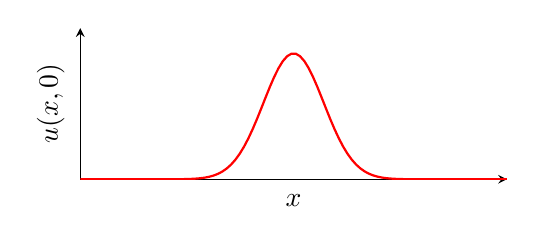
\begin{tikzpicture}
      \begin{axis}[
        axis lines = left,
        xlabel = $x$,
        ylabel = {$u(x, 0)$},
        domain=0:10,
        samples=100,
        ymin=0, ymax=1.2,
        xtick=\empty,
        ytick=\empty,
        width=7cm,
        height=3.5cm,
      ]
        \addplot[thick, red] {exp(-((x-5)^2))};
      \end{axis}
    \end{tikzpicture}
    \caption{Initial heat distribution, concentrated at the center like a drop of ink.}
  \end{subfigure}
  \hfill
  \begin{subfigure}[t]{0.45\textwidth}
    \centering
    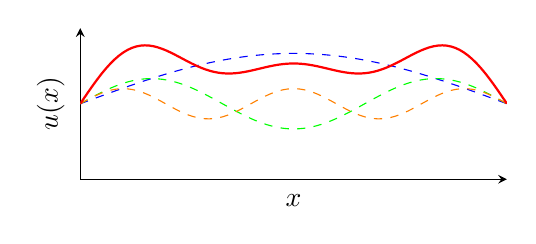
\begin{tikzpicture}
      \begin{axis}[
        axis lines = left,
        xlabel = $x$,
        ylabel = {$u(x)$},
        domain=0:10,
        samples=100,
        ymin=-1.5, ymax=1.5,
        xtick=\empty,
        ytick=\empty,
        width=7cm,
        height=3.5cm,
      ]
        \addplot[blue, dashed] {sin(deg(pi*x/10))};
        \addplot[green, dashed] {0.5*sin(deg(3*pi*x/10))};
        \addplot[orange, dashed] {0.3*sin(deg(5*pi*x/10))};
        \addplot[thick, red] {sin(deg(pi*x/10)) + 0.5*sin(deg(3*pi*x/10)) + 0.3*sin(deg(5*pi*x/10))};
      \end{axis}
    \end{tikzpicture}
    \caption{The initial profile as a sum of sine waves of different frequencies.}
  \end{subfigure}

  \vspace{0.8cm}

  % Second row: Time evolution and final state
  \begin{subfigure}[t]{0.45\textwidth}
    \centering
    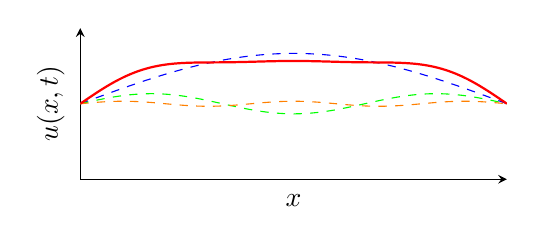
\begin{tikzpicture}
      \begin{axis}[
        axis lines = left,
        xlabel = $x$,
        ylabel = {$u(x, t)$},
        domain=0:10,
        samples=100,
        ymin=-1.5, ymax=1.5,
        xtick=\empty,
        ytick=\empty,
        width=7cm,
        height=3.5cm,
      ]
        \addplot[blue, dashed] {sin(deg(pi*x/10))};
        \addplot[green, dashed] {0.2*sin(deg(3*pi*x/10))};
        \addplot[orange, dashed] {0.05*sin(deg(5*pi*x/10))};
        \addplot[thick, red] {sin(deg(pi*x/10)) + 0.2*sin(deg(3*pi*x/10)) + 0.05*sin(deg(5*pi*x/10))};
      \end{axis}
    \end{tikzpicture}
    \caption{Over time, high-frequency components decay faster.}
  \end{subfigure}
  \hfill
  \begin{subfigure}[t]{0.45\textwidth}
    \centering
    \begin{tikzpicture}
      \begin{axis}[
        axis lines = left,
        xlabel = $x$,
        ylabel = {$u(x, t \to \infty)$},
        domain=0:10,
        samples=2,
        ymin=0, ymax=1.2,
        xtick=\empty,
        ytick=\empty,
        width=7cm,
        height=3.5cm,
      ]
        \addplot[thick, blue] coordinates {(0,0.4) (10,0.4)};
      \end{axis}
    \end{tikzpicture}
    \caption{Eventually, the temperature becomes uniform.}
  \end{subfigure}

  \caption{Fourier analysis of heat flow: from initial condition to spectral decomposition and smoothing over time.}
\end{figure}


He understood that sine and cosine functions possess a special property called orthogonality. In simple terms, this means that when you compare different sine and cosine waves over a complete cycle — say, by calculating how much they "overlap" through integration — their contributions to each other cancel out perfectly. They’re like two dancers moving in rhythm but on completely different paths: one moves side-to-side, the other up-and-down, and no matter how long you watch them, their motions never reinforce or interfere with each other.

Mathematically, this orthogonality means that if you multiply, for example, a sine wave and a cosine wave of the same frequency and integrate the result over a full period (like one full oscillation), you get zero. It’s as if one wave is completely “invisible” to the other when measuring energy or contribution across time.

You can think of this like tuning forks that vibrate at different frequencies — strike one, and the others don’t resonate unless they’re tuned the same way. Or imagine shining red and green lights onto a screen: their colors don’t mix unless you explicitly combine them. Similarly, in the Fourier series, each sine and cosine function only captures its own frequency component — it ignores everything else. That’s what makes them such a powerful basis for building up complicated waveforms: each part contributes cleanly and independently, without muddying the signal.

This insight is what allows Fourier series to break down any periodic function into a clean sum of sinusoids — each part precisely measures just one "ingredient" in the recipe, with no cross-talk between them.

\begin{figure}[H]
    \centering
    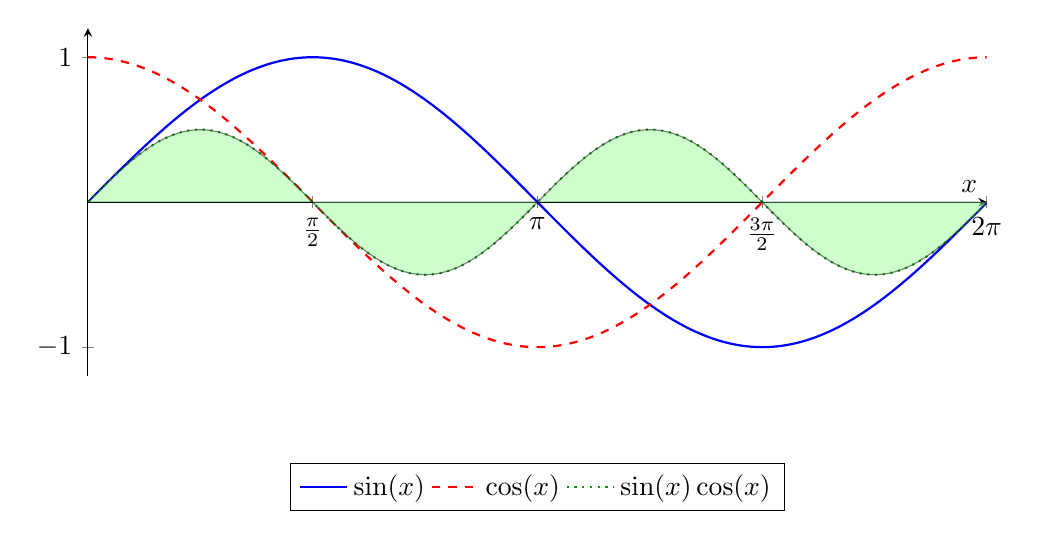
\begin{tikzpicture}
        \begin{axis}[
            width=13cm,
            height=6cm,
            axis lines=middle,
            xlabel={$x$},
            ylabel={},
            xtick={0, 1.57, 3.14, 4.71, 6.28},
            xticklabels={$0$, $\frac{\pi}{2}$, $\pi$, $\frac{3\pi}{2}$, $2\pi$},
            ytick={-1,0,1},
            ymin=-1.2, ymax=1.2,
            samples=300,
            domain=0:6.28,
            legend style={at={(0.5,-0.25)}, anchor=north, legend columns=3},
            clip=true,
        ]
            % sin(x)
            \addplot [blue, thick] {sin(deg(x))};
            % cos(x)
            \addplot [red, thick, dashed] {cos(deg(x))};
            % sin(x)cos(x)
            \addplot [green!60!black, thick, dotted] {sin(deg(x))*cos(deg(x))};

            % Fill positive area
            \addplot [
                domain=0:pi,
                fill=green!40,
                opacity=0.5,
            ] {sin(deg(x))*cos(deg(x))} \closedcycle;

            % Fill negative area
            \addplot [
                domain=pi:2*pi,
                fill=green!40,
                opacity=0.5,
            ] {sin(deg(x))*cos(deg(x))} \closedcycle;

            \legend{$\sin(x)$, $\cos(x)$, $\sin(x)\cos(x)$}
        \end{axis}
    \end{tikzpicture}
    \caption{Orthogonality of $\sin(x)$ and $\cos(x)$: The product $\sin(x)\cos(x)$ has symmetric positive and negative areas over $[0, 2\pi]$, which cancel out when integrated.}
    \label{fig:sin_cos_cancellation}
\end{figure}



But the implications of this went far beyond heat. If any function could be expressed as an infinite sum of sines and cosines, what did that mean for functions that weren’t so well-behaved? Could even jagged, discontinuous functions be decomposed into smooth waves? 

Fourier’s answer was yes. And that’s when things got weird.

\subsection{The Square Wave: A Function That Shouldn’t Exist}

Consider the \textbf{square wave function}, a simple periodic function that jumps suddenly between two values:

\[
f_{\text{square}}(x) =
\begin{cases}
    1, & -\pi < x < 0 \\
   -1, & 0 < x < \pi
\end{cases}
\]

\begin{center}
\begin{tikzpicture}
    \begin{axis}[
        domain=-2*pi:2*pi,
        samples=100,
        axis x line=middle,
        axis y line=middle,
        ymin=-1.5, ymax=1.5,
        xlabel={$x$}, ylabel={$f(x)$},
        xtick={-6.28, -3.14, 0, 3.14, 6.28},
        xticklabels={$-2\pi$, $-\pi$, $0$, $\pi$, $2\pi$},
        title={Square Wave Function}
    ]

        % Square wave segments
        \addplot[thick] coordinates {(-2*pi,-1) (-pi,-1)};
        \addplot[thick] coordinates {(-pi,1) (pi,1)};
        \addplot[thick] coordinates {(pi,-1) (2*pi,-1)};
        
        % Vertical jumps to indicate discontinuities
        \addplot[thick, dashed] coordinates {(-pi,-1) (-pi,1)};
        \addplot[thick, dashed] coordinates {(pi,1) (pi,-1)};

        % Open circles (discontinuities)
        \node at (axis cs: -pi,-1) {\textcolor{black}{$\circ$}};
        \node at (axis cs: pi,1) {\textcolor{black}{$\circ$}};

        % Filled circles (function is defined at these points)
        \filldraw[black] (axis cs: -pi,1) circle (2pt);
        \filldraw[black] (axis cs: pi,-1) circle (2pt);

    \end{axis}
\end{tikzpicture}
\end{center}

Suddenly, the comforting idea that “nice functions behave nicely” was thrown into chaos. Functions with violent, unnatural jumps were somehow being rebuilt using nothing but smooth sine waves, and worse—those waves weren’t even behaving the way mathematicians expected. Instead of politely smoothing out the discontinuities, the Fourier series doubled down on the absurdity.

Here’s what made everyone question their life choices:

\begin{itemize}
    \item The right-hand side of the equation consists \textbf{only of smooth sine waves}.
    \item The left-hand side is a function with \textbf{sharp jumps (discontinuities)} at \( x = 0, \pm \pi \).
    \item Despite being an \textbf{infinite sum of smooth functions}, the Fourier series does \textbf{not smooth out the jump}.
    \item Instead, the series converges to the discontinuity but introduces oscillations, an effect now known as the \textbf{Gibbs phenomenon}.
\end{itemize}

This result was a major paradigm shift. It revealed that Fourier series could approximate functions far beyond the class of smooth, differentiable functions, forcing mathematicians to rethink fundamental assumptions about convergence, function representation, and the very nature of mathematical analysis.
